
\section{Discussion}
\label{sec:discussion}




\begin{figure*}[t!]
  \centering
  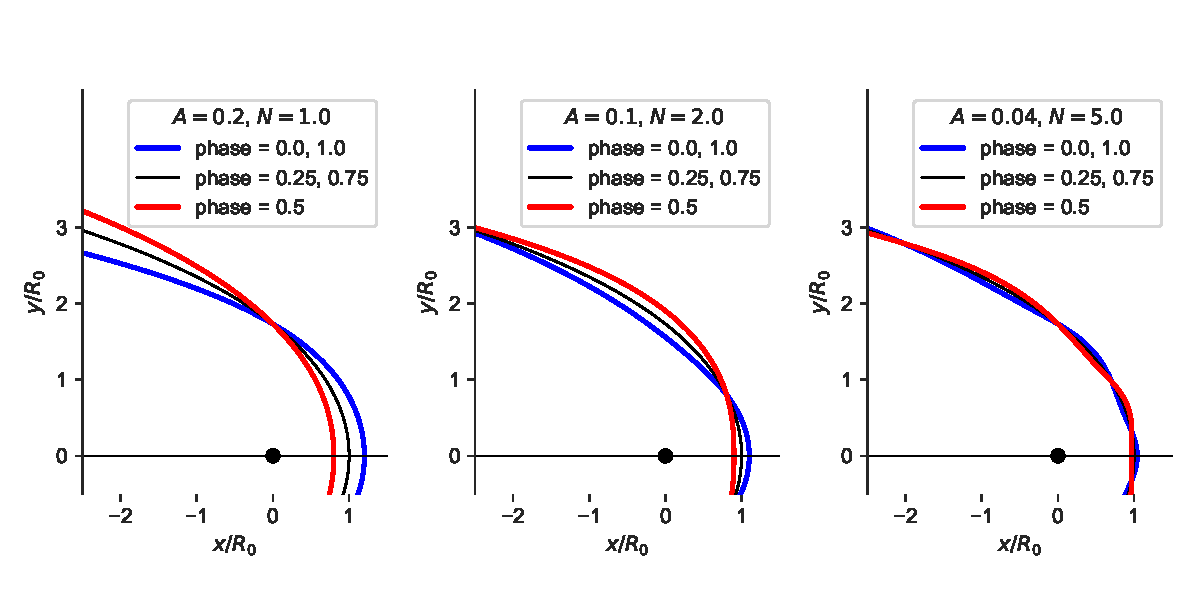
\includegraphics[width=\linewidth]{figs/compare_xyprime_wave-wilkinoid}
  \caption{Small-amplitude standing wave perturbations to wilkinoid
    bow shapes.  The maximum deviations from the base shape are seen
    at phases \(\phi = 0\) (blue line) and \(\phi = 0.5\) (red line), while
    the perturbation is zero at \(\phi = 0.25\) and \(0.75\) (black
    line).  Results are shown left to right for increasing wave
    numbers \(N\) and decreasing amplitudes \(A\): (a)~\(A = 0.1\),
    \(N = 1.0\), (b)~\(A = 0.05\), \(N = 2.0\), (a)~\(A = 0.02\),
    \(N = 5.0\).}
  \label{fig:perturb-shapes}
\end{figure*}

% \begin{figure*}
%   \centering
%   \includegraphics[width=\linewidth]
%   {figs/wave_xyprime-A005-N20-ancantoid-xi080-beta000500}
%   \caption{Plane-of-sky projections of perturbed bow shapes.  In all
%     cases, the base bow shape is ancantoid with \(\xi = 0.8\),
%     \(\beta = 0.005\) and the perturbation is the same as in the central
%     panel of Fig.~\ref{fig:perturb-shapes}, with amplitude
%     \(A = 0.05\) and wave number \(N = 2.0\). Results are shown for
%     inclination angles \(i = 0\) to \(i = 75^\circ\) (indicated by line
%     color and thickness, see key) and for different fractional phases
%     of the oscillation: (a)~\(\varphi = 0.0\), (b)~\(\varphi = 0.25\),
%     (c)~\(\varphi = 0.50\). Unlike in Fig.~\ref{fig:perturb-shapes},
%     the spatial coordinates are normalized to the instantaneous
%     projected apex radius \(R_0'\) at each phase, so the apex does not
%     appear to move.}.
%   \label{fig:perturb-xy-prime}
% \end{figure*}

\subsection{Perturbed bows}
\label{sec:perturbed-bows}

Instability of bow \citep{Blondin:1998a}

The bow shock models that we have considered so far have been
steady-state: although material is moving throughout the bow, the
pattern of its structure does not vary with time.  In this section, we
consider small, time-varying perturbations to such a steady-state
structure.  These may be due to periodic variations in the
momentum-loss rate of one of the winds, or due to dynamical
instabilities in the shocked shell.

We consider fractional perturbations \(\Delta(\theta, t)\) of a base shape
\(R(\theta)\), such that
\(R(\theta) \to [1 + \Delta(\theta, t)] R(\theta)\).  For simplicity,
\(\Delta(\theta, t)\) is a standing wave of constant amplitude \(A\), which is
periodic in \(\theta\), with wave number \(N\).  In cylindrical symmetry
\(\Delta(\theta, t)\) must be even in \(\theta\), so can be expressed as
\begin{equation}
  \label{eq:standing-wave}
  \Delta(\theta, t) = A \cos(N \theta) \cos(2\pi \varphi) . 
\end{equation}
For waves with period \(P\), the fractional phase \(\varphi\) will
vary with time \(t\) as
\begin{equation}
  \label{eq:fractional-phase}
  \varphi(t) = (\varphi_0 + t/P) \bmod 1.0\ ,
\end{equation}
where \(\varphi_0\) is an arbitrary reference phase.

Example oscillations with wave numbers \(N = 1.0\), \(2.0\), and
\(5.0\) superimposed on a wilkinoid base shape are shown in
Figure~\ref{fig:perturb-shapes}.  There are \(N\) nodes of the
oscillation between \(\theta = [0, \pi]\), always with an antinode at the apex
(\(\theta = 0\)), as required by symmetry.  So, with \(N = 1.0\) there is a
node (fixed point) in the near wing at \(\theta = \pi/2\), but an antinode in
the far wing at \(\theta = \pi\), which is in antiphase with the oscillation
of the apex, giving rise to a large-scale ``breathing'' mode of
oscillation.  With \(N = 2.0\), there are nodes at \(\theta = \pi/4\) and
\(3\pi/4\), while the antiphase antinode has moved to the near wing at
\(\theta = \pi/2\).  There is still an antinode in the far wing at
\(\theta = \pi\) but it is now in phase with the apex, giving rise to a
``curling-up/straightening-out'' mode of oscillation.  With
\(N = 5.0\), there are many more nodes and antinodes, giving a
``ringing'' mode of oscillation.  Note that all our examples have
\(A \propto 1/N\) in order to keep the local curvature relatively low.  If
the product \(A N\) is not small compared to unity, then the local
curvature can be so extreme as to reverse the concave shape of the
base bow shape, producing locally convex regions.

If the bow shape is viewed at different inclinations, then the effect
of the oscillations on the projected shape will vary.  In particular,
the apex-to-wing interval in body-frame angle changes from
\(\theta = [0, \pi/2]\) at \(i = 0\) to
\(\theta = [\theta_0, \theta_{90}]\) for general \(i\), see
equations~\eqref{Q-eq:thetapar} and \eqref{Q-eq:th90} of \PaperI{}.
The difference \(\theta_{90} - \theta_0\) is always a declining function of
\(|i|\), so the oscillations of the tangent line become increasingly
stretched out as the inclination increases.  This effect can be seen
in Figure~\ref{fig:perturb-xy-prime}, which shows an example of the
variation in projected perturbed shape with inclination angle for 3
different phases, this time for an ancantoid base shape and the
\(N = 2.0\) perturbation shown in Figure~\ref{fig:perturb-shapes}b.
The most marked changes with phase are seen for low inclinations,
whereas the changes are smaller, although still noticeable, for
\(|i| \ge 45^\circ\). If \(A N\) exceeds about 0.5, then the local curvature
of the perturbations is so extreme that multiple tangent lines exist
at intermediate inclinations, which produces the appearance of
additional incomplete bright arcs inside the main arc of the bow.

\begin{figure}
  \centering
  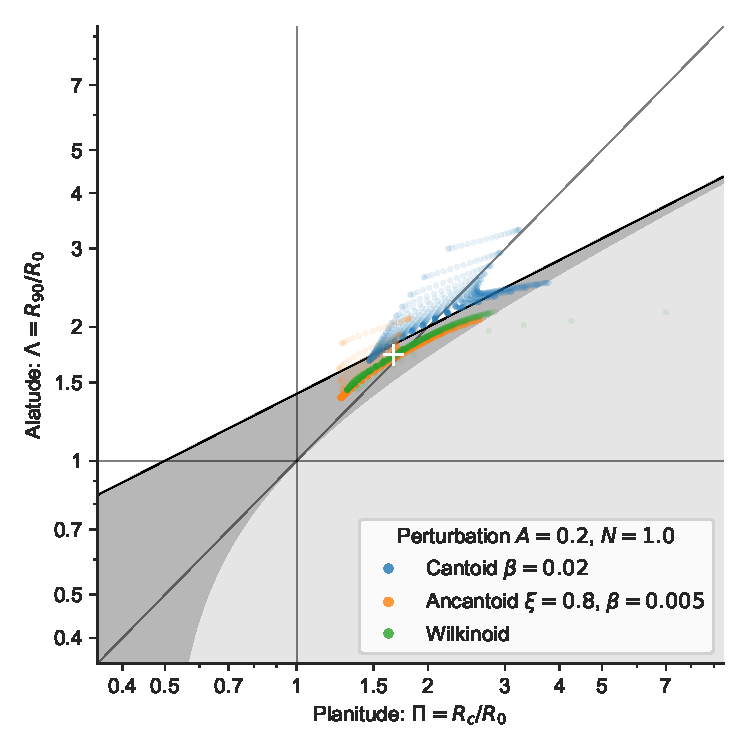
\includegraphics[width=\linewidth]
  {figs/wave-R90-vs-Rc-A020-N10}
  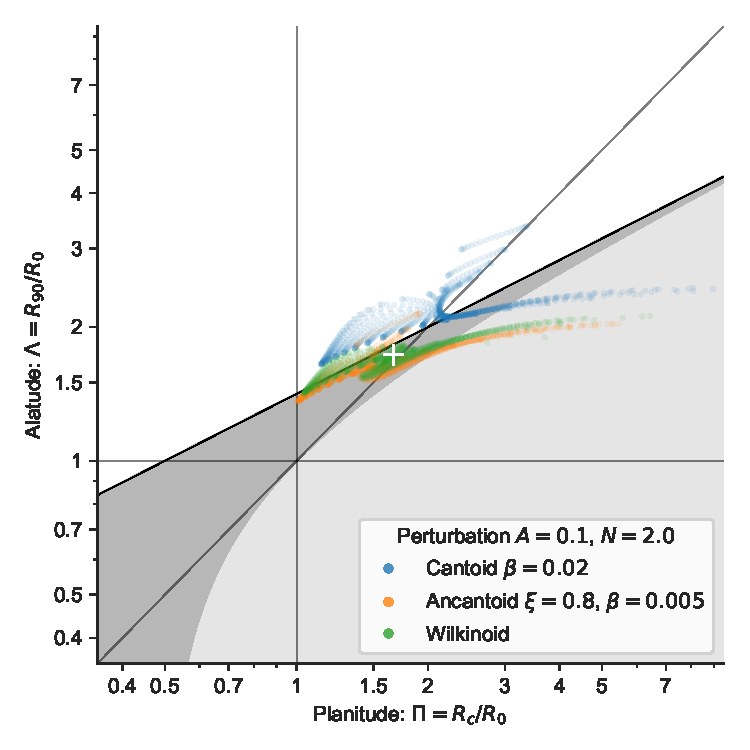
\includegraphics[width=\linewidth]
  {figs/wave-R90-vs-Rc-A010-N20}
  \caption{Diagnostic diagram for perturbed shapes}
  \label{fig:perturb-Rc-R90}
\end{figure}



%%% Local Variables:
%%% mode: latex
%%% TeX-master: "obs-bowshocks"
%%% End:
